\documentclass[10pt]{article} 
\usepackage[margin=0.6in]{geometry}
\usepackage{wasysym}
\usepackage{setspace} 
\usepackage{graphicx} 
\usepackage{caption}
\usepackage{multicol}
\usepackage{subcaption} 
\usepackage{array} 
\usepackage{booktabs}
\usepackage{listings} 
\usepackage{float}
\usepackage{enumitem}
\usepackage{lmodern}    
\usepackage{xcolor}
\lstset{
    language=C++,
    basicstyle=\ttfamily\footnotesize,
    keywordstyle=\color{blue},
    stringstyle=\color{red},
    commentstyle=\color{green},
    morecomment=[l][\color{magenta}]{\#},
    numbers=left,
    numberstyle=\tiny\color{gray},
    stepnumber=1,
    numbersep=10pt,
    showspaces=false,
    showstringspaces=false,
    tabsize=4,
    breaklines=true,
    breakatwhitespace=false,
}
\setstretch{1.5}

\title{Design Process of Room Temperature Monitor} \author{Giacomo Cappelletto\\ BU ID: U91023753} % leave empty to omit date
\date{}
\begin{document}

\maketitle

\section{Summary}

\noindent
This report presents a portable room temperature monitor built with a TMP36
sensor and Arduino Uno, displaying readings on a $16\times2$
I\textsuperscript{2}C LCD and triggering LEDs and a buzzer when a
running-average setpoint is exceeded. It outlines the design approachsensor
integration, firmware development, circuit assembly, and custom enclosure CAD
modeling, The key outcomes of this project: $\pm 0.5^{\circ}C$ linear accuracy
over the operational range and approximately 6.7 h runtime on a single 9 V
battery. These results demonstrate a low-cost, energy-efficient solution for
real-time temperature monitoring and alerting.
\section{Introduction}

Maintaining a comfortable and stable indoor temperature
is crucial to modern building management and directly impacts both energy
consumption as well as the wellbeing of those who occupy it. Traditional thermostats regulate heating and
cooling systems based on set threshold temperatures, but commercial units can be costly
and therefore inaccessible for small-scale or experimental applications. In response to
growing concerns over energy efficiency and sustainability, it is important to
explore low-cost, modular solutions that allow fine-grained temperature
monitoring and control in real world environments.

This project addresses the need for an accessible, do-it-yourself room
temperature monitoring system by integrating a TMP36 analog temperature sensor,
a $16\times 2$ I\textsuperscript{2}C LCD, and an Arduino UNO microcontroller. By
automating the measurement and display of ambient temperature, the device can
inform control actions in the event loop (such as triggering a fan or heater),
enabling users to avoid over-adjusting the temperature in their spaces, reducing
unnecessary energy use. A $9\,$V battery, switch, green and red LEDs, and a
buzzer provide basic power, status indication, and alerts without reliance on
wall plug electricity.

This project has two main aims: first, to replicate the core functionality of a
simple thermostat using components and techniques covered in our course. Second,
to develop skills in assembling electronic hardware, writing
microcontroller code (in C++), and designing enclosures in CAD. For that part of the project
enclosure, lid, battery holder, and internal baseplate were modeled and
fabricated to store and organize all components, wired using $22$ AWG and
female-to-female jumper cables for I\textsuperscript{2}C data connections.

The purpose of this report is to document the design process, from component
selection and design to circuit assembly and firmware development, and
to evaluate the system's performance against expected objectives. By following
the design methodology outlined here, we demonstrate how simple and
easily sourceable parts can be combined into a cohesive temperature
monitoring tool.


\section{Design elements} Explain your design decisions. Address each of the
following:

\begin{enumerate}[label=\Alph*.]
	\item \textbf{List Of Used Components}
	      \begin{multicols}{2}
		      \begin{itemize}
			      \item 1 $\times$ Injection Mold ABS Enclosure (Bottom and Lid)
			      \item 1 $\times$ Transparent Acrylic Lase Cut Base Plate
			      \item 8 $\times$ Polycarbonate Flat Top Phillips Screws
			      \item 8 $\times$ Polycarbonate Bolts
			      \item 8 $\times$ Metal Round Head Phillips Screws
			      \item 8 $\times$ Plastic 0.5 mm spacers
			      \item 1 $\times$ $9 V$ Battery
			      \item 1 $\times$ PLA FDM Printed $9 V$ Battery holder
			      \item 1 $\times$ Arduino UNO microcontroller
			      \item 1 $\times$ Alphanumeric $16 \times 2$ I\textsuperscript{2}C LCD with IIC
			      \item 1 $\times$ TMP36 Analog Temperature sensor
			      \item 1 $\times$ Piezo Capsule Buzzer
			      \item 1 $\times$ Red LED
			      \item 1 $\times$ Green LED
			      \item 1 $\times$ 2 way switch
			      \item 2 $\times$ Female-Female $4''$ jumper wires
			      \item 15 $\times$ $6''$ 22 AWG Wires (White and Red)
			      \item 1 $\times$ $220 \Omega$ resistor
			      \item 1 $\times$ $1 k\Omega$ resistor
			      \item 2 $\times$ Twist Nut Caps
			      \item 2 $\times$ Spade Connectors
		      \end{itemize}
	      \end{multicols}
	\item \textbf{Precision measurements}
	      \begin{table}[H]
		      \centering
		      \caption{Relevant dimensions of major components (see Appendix A for Figures \ref{fig:1-c} - \ref{fig:7-c})}
		      \label{tab:dim_condensed}
		      \begin{tabular}{l c c c c c}
			      \toprule
			      Item                                               & Fig.\ ID                & W [mm] & L [mm] & H [mm] & $\diameter $ [mm] \\
			      \midrule
			      Full Assembly                                      & \ref{fig:full_assembly} & 123,8  & 146,1  & 63,1   & -                 \\
			      Injection Mold ABS Enclosure Bottom                & \ref{fig:1-c}           & 119,0  & 146,1  & 57,4   & -                 \\
			      Injection Mold ABS Enclosure Lid                   & \ref{fig:2-c}           & 119,0  & 120,1  & 5,5    & -                 \\
			      Transparent Acrylic Laser-Cut Base Plate           & \ref{fig:3-c}           & 95,0   & 96,1   & 9,0    & -                 \\
			      Arduino UNO Microcontroller                        & \ref{fig:4-c}           & 53,3   & 74,9   & 15,2   & -                 \\
			      9 V Battery and PLA-Printed Holder                 & \ref{fig:5-c}           & 29,7   & 48,8   & 21,0   & -                 \\
			      Alphanumeric $16\times2$ I\textsuperscript{2}C LCD & \ref{fig:6-c}           & 36,0   & 80,0   & 22,0   & -                 \\
				  TMP36 Analog Temperature Sensor                    & \ref{fig:7-c}           & -      & -      & 14,6   & 2,5               \\
			      \bottomrule
		      \end{tabular}
		      \begin{center}
			      \textit{Full Table in Appendix (see Section \ref{sec:full_table})}
		      \end{center}
	      \end{table}
	      \pagebreak
	\item \textbf{CAD drawings}
	      \begin{figure}[H] \centering
		      \includegraphics[width=0.5\textwidth]{cad/c-c.jpeg}
		      \caption{CAD assembly of the prototype.}
		      \label{fig:full_assembly}
	      \end{figure}


	      \begin{center}
		      \textit{Figures \ref{fig:1-c} - \ref{fig:7-c} in Appendix (see Section \ref{sec:appendixA})}
	      \end{center}



	\item \textbf{Prototype photographs}
	      \begin{figure}[H] \centering
		      \begin{subfigure}[b]{0.45\textwidth}
			      \centering
			      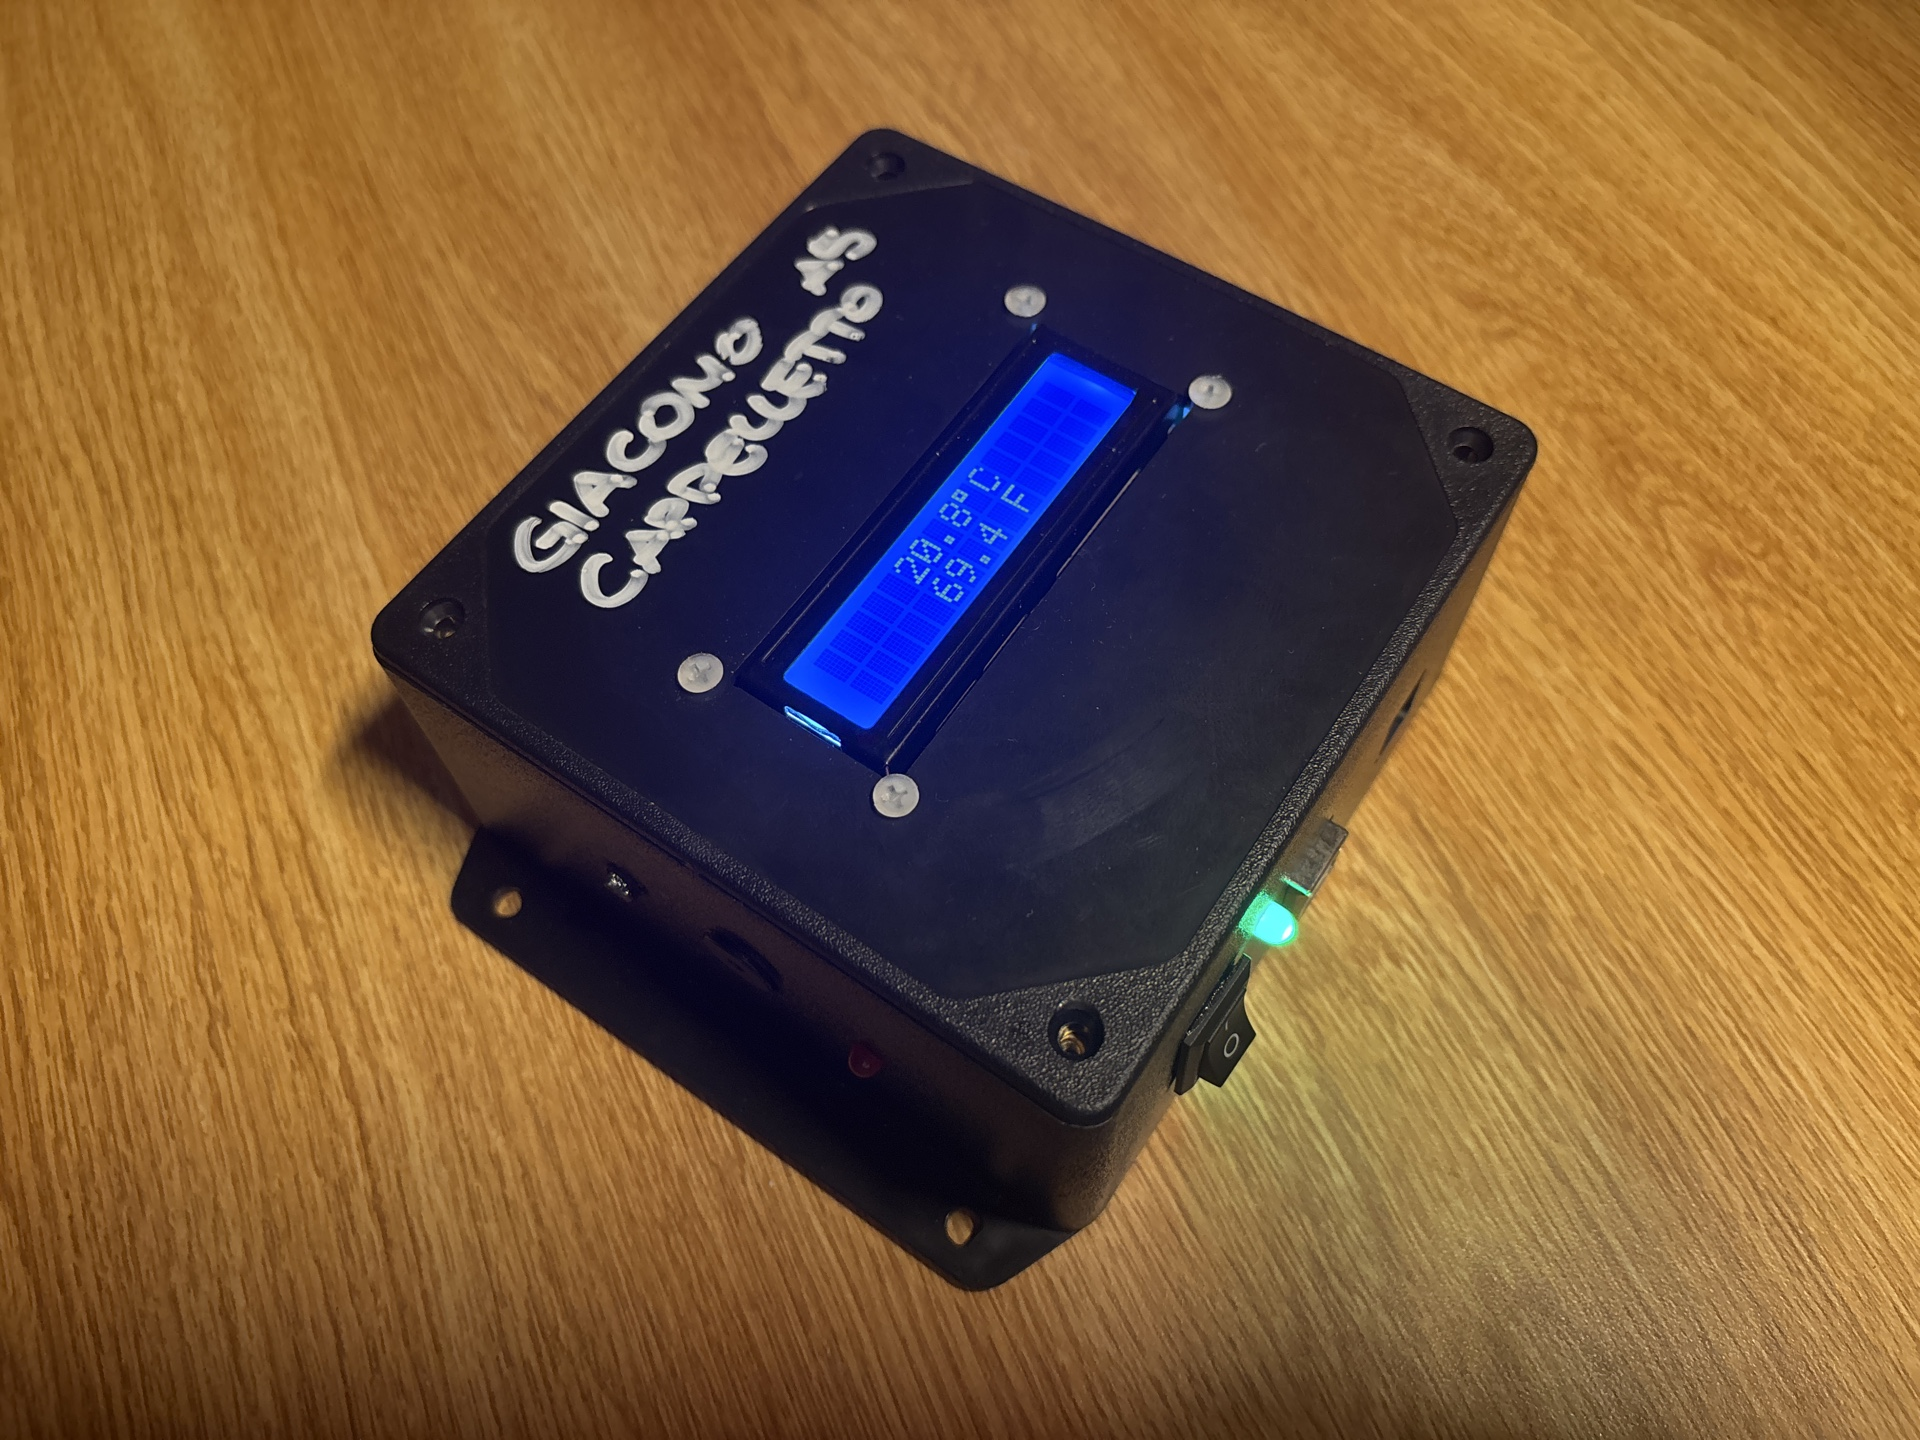
\includegraphics[width=0.7\textwidth]{cad/f-1.jpeg}
			      \caption{With lid}
		      \end{subfigure} \hfill
		      \begin{subfigure}[b]{0.45\textwidth}
			      \centering
			      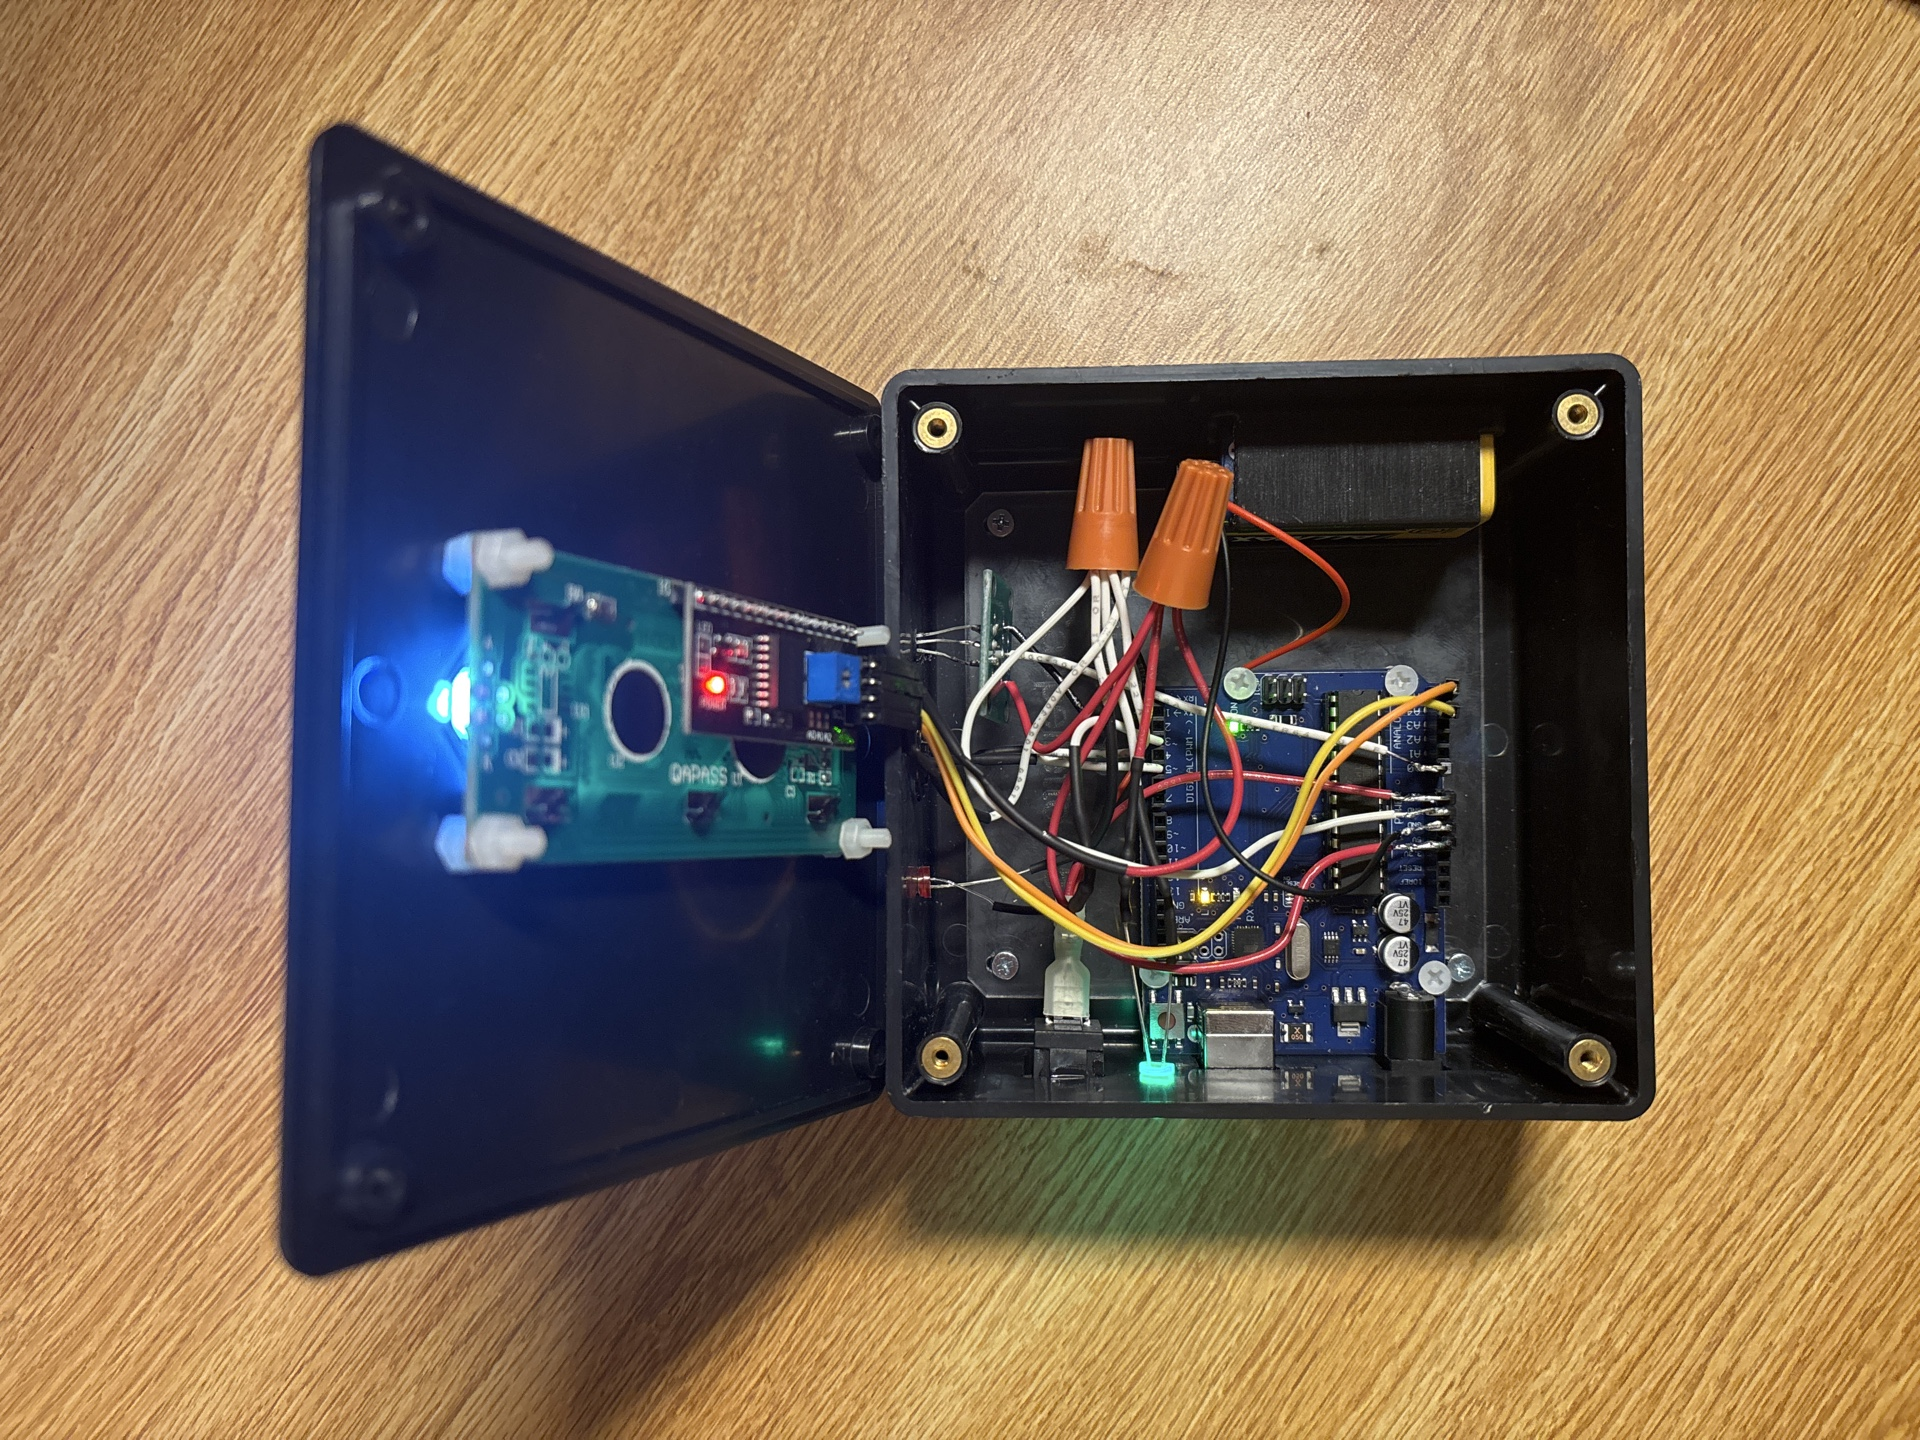
\includegraphics[width=0.7\textwidth]{cad/f-2.jpeg}
			      \caption{Without lid}
		      \end{subfigure}
		      \caption{Top views of the working prototype.}
	      \end{figure}


	\item \textbf{Purpose of using an Arduino board}

	      In this project, the Arduino UNO serves as the central controller: it
	      reads the TMP36's analog voltage on pin A0 using its 10-bit ADC
	      ($0-1023$ counts for $0-5V$), converts that value to temperature in °C
	      and °F, and drives the $16\times2$ I\textsuperscript{2}C LCD over
	      SDA/SCL (pins A4/A5) via the LiquidCrystal\_I2C library. Inside the
	      \texttt{loop()} function (sampling once per second), the firmware
	      compares the measured running average temperature (over 5 seconds)
	      against a setpoint and, when thresholds are crossed, toggles digital
	      pin D3 to light the red (220 $\Omega$ series) LED and pulses pin D4 to
	      sound the buzzer. This programmable feedback mechanism both displays
	      real-time readings and issues visual/audible alerts, all managed by
	      the Arduino's microcontroller. Furthermore, we are able to execute
	      arithmetic operations such as the running average of the temperature
	      over a set interval, effectively addressing the initial issue of over
	      regulation of temperature in thermostats.

	      \pagebreak
	\item \textbf{Wiring diagram and methods}

	      \begin{figure}[H]
		      \centering
		      \begin{minipage}[c]{0.48\textwidth}
			      \centering
			      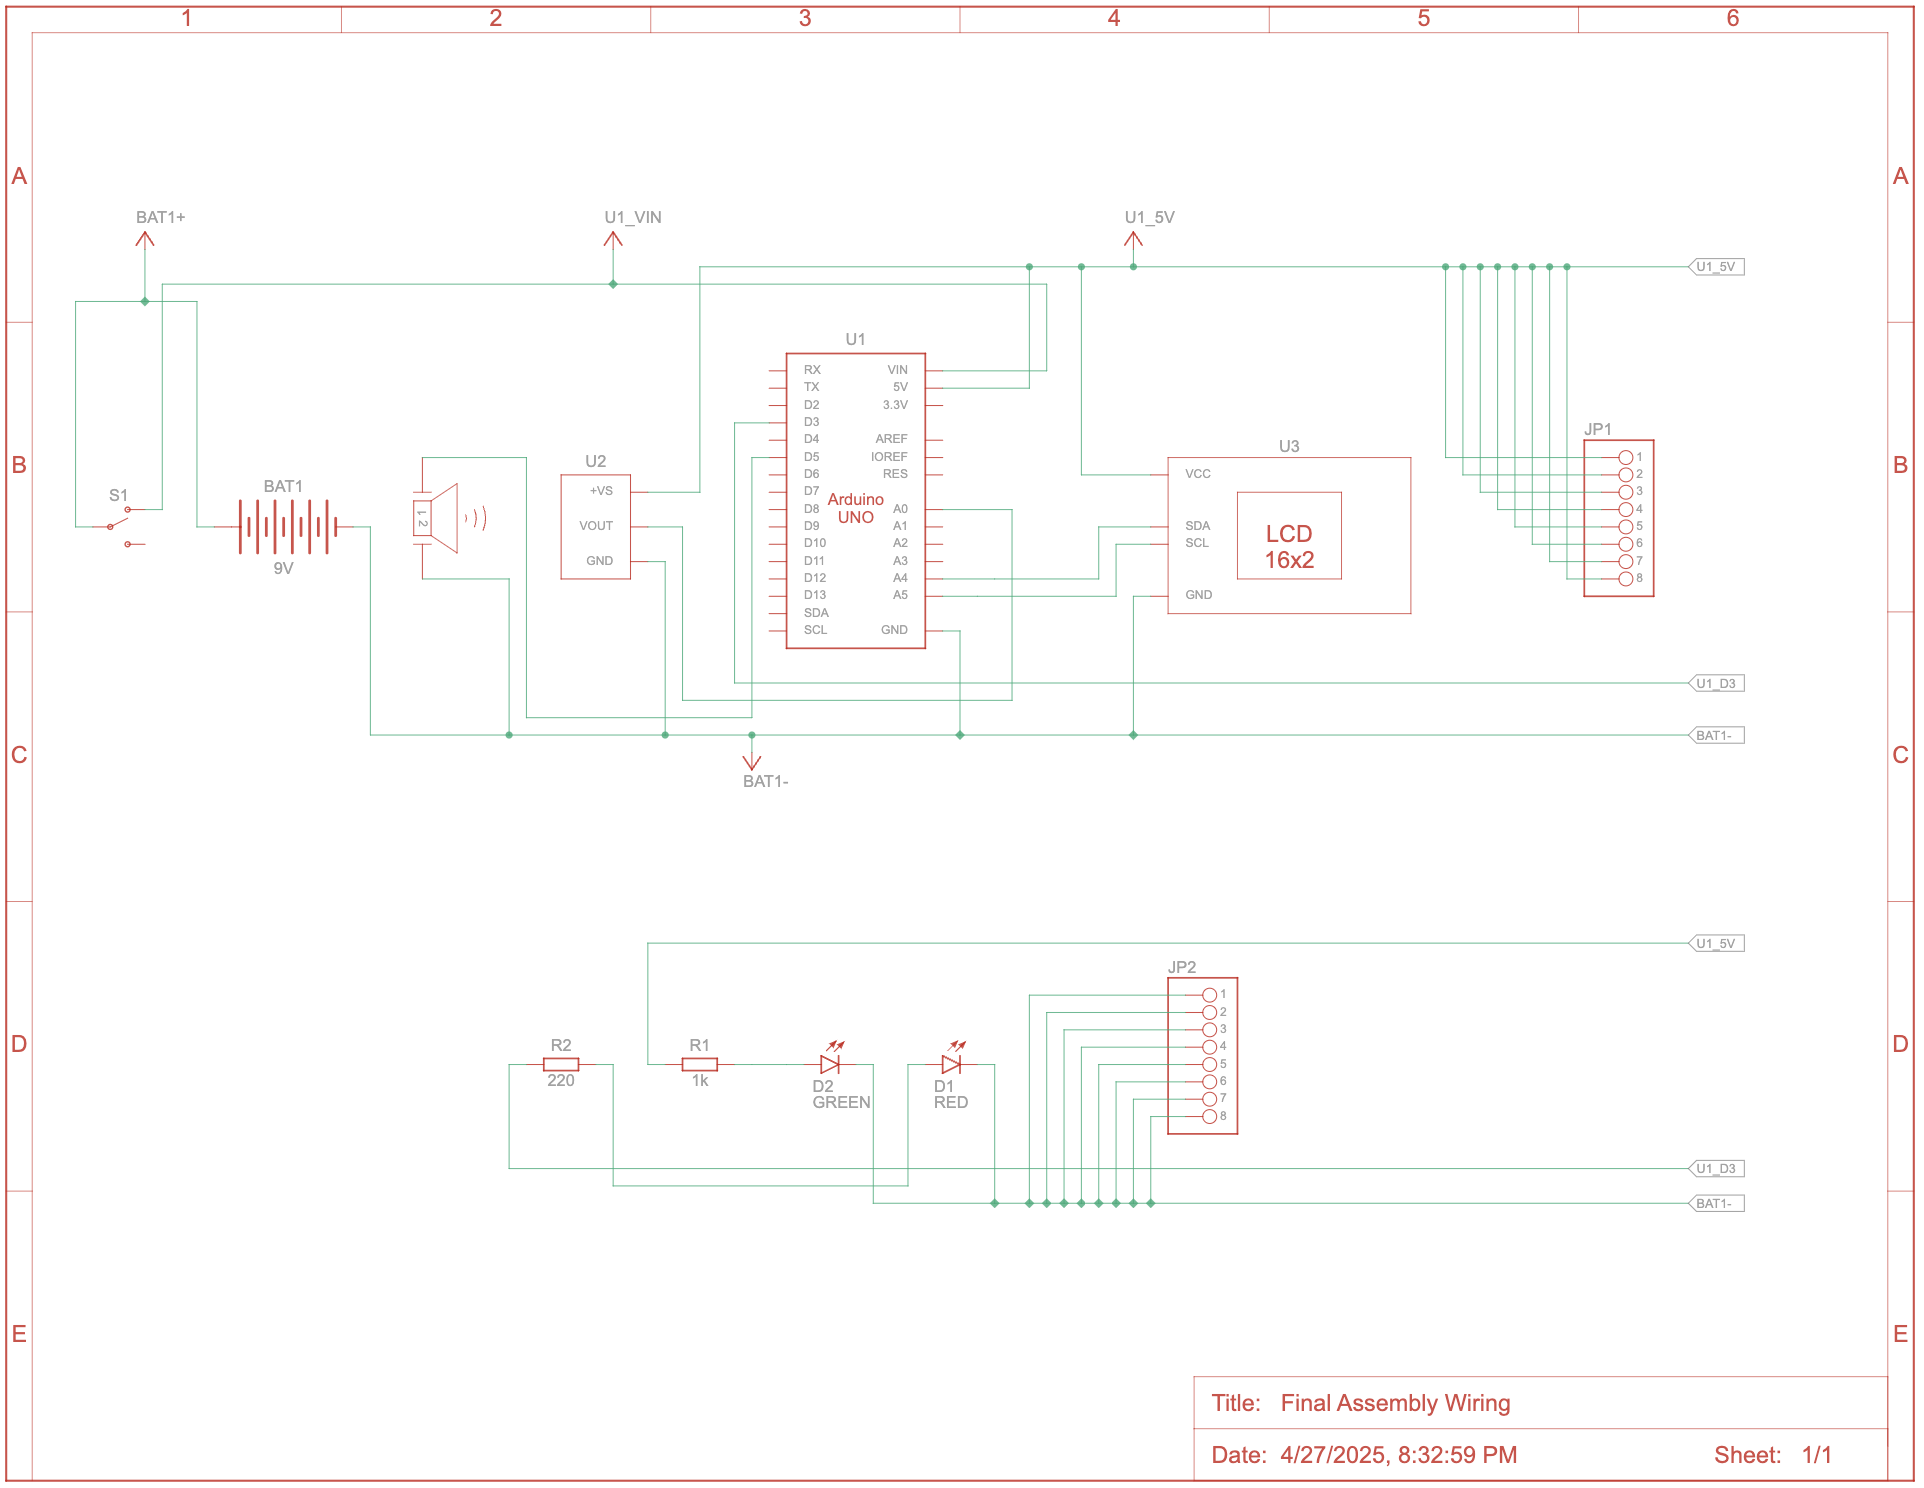
\includegraphics[width=\linewidth]{cad/w-c.png}
			      \captionof{figure}{Circuit wiring diagram.}
			      \label{fig:w-c}
		      \end{minipage}\hfill
		      \begin{minipage}[c]{0.48\textwidth}
			      Figure~\ref{fig:w-c} shows the final assembly. All GND and positive lines, as
			      well as the analog TMP36, are soldered to 90° male header pins on the Arduino Uno
			      for a secure, low-profile connection. The SDA/SCL lines to the $16\times2$
			      I\textsuperscript{2}C LCD use female-female jumper wires for easy removal.
			      Two twist-on wire nuts combine the multiple battery positive and negative leads,
			      permitting quick disassembly and reconfiguration. The power switch is fitted
			      with insulated spade connectors to maintain a clean, removable interface.
		      \end{minipage}
	      \end{figure}



	\item \textbf{Wire gauge and resistor values} \label{sec:wires}

	      All main power and signal lines use 22 AWG to keep series resistance low and provide good strength since the LCD lines need to bend when removing the lid. The I\textsuperscript{2}C SDA/SCL connections use thinner jumper wires (26 AWG) since their $< 1 m \, A$ currents tolerate higher resistance and allow quick reconnection.\\
	      Series resistors: green LED $R_G=1k\Omega$, red LED $R_R=220\,\Omega$.\\
	      By KVL in each LED loop:
	      \[
		      5 V - I_G R_G - V_{F,G}=0
		      \quad\Longrightarrow\quad
		      I_G=\frac{5-2.1}{1000} = 2.9 \, mA,
	      \]
	      \[
		      5V - I_R R_R - V_{F,R}=0
		      \quad\Longrightarrow\quad
		      I_R=\frac{5-2.0}{220} = 13.6 \, mA,
	      \]
	      where $V_{F,G}=2.1\,$V and $V_{F,R}=2.0\,$V are the LED forward voltages.

	\item \textbf{Internal power supply} A $9\,$V battery was chosen for its
	      compact size, ease of integration and replacement. Typical 9 V batteries
	      have a capacity of $C\approx500\,$mAh. Given the device's draw (as per DMM) are
	      \[
		      I_{\mathrm{avg}} \approx I_{\mathrm{Arduino}} +
		      I_{\mathrm{LCD}} + I_{\mathrm{TMP+LEDs}} \approx
		      50\mathrm{\,mA}+20\mathrm{\,mA}+5\mathrm{\,mA}=75\mathrm{\,mA},
	      \]
	      the expected runtime $t$ is
	      \[
		      t = \frac{C}{I_{\mathrm{avg}}} =
		      \frac{500\mathrm{\,mAh}}{75\mathrm{\,mA}} \approx 6.7 h
	      \]
	      This is ok for a
	      prototype, but would be unusable for real world applications, as users would
	      need to replace the devices power supply up to 4 times a day.  For longer
	      operation, the Arduino can be powered externally via the barrel jack (7-12
	      V) or USB/USB-C 5V input.

	\item \textbf{Arduino code}


	      \begin{center}
		      \textit{See Appendix for code (Section \ref{sec:code})}
	      \end{center}

	\item \textbf{Prototype specifications}

	      \begin{itemize}
		      \item Voltage of power supply: $9\,$V
		      \item Operating voltage of circuit: $5\,$V
		      \item Total current drawn (measured with DMM): $\approx75\,$mA
		      \item Battery operating time: $\displaystyle t = \frac{C}{I_{\mathrm{avg}}}\approx6.7 h$ as previously shown
		      \item Sensor temperature range (from datasheet): $-40\,$°C to $125\,$°C
		      \item Comfortable temperature range: $20\,$°C to $25\,$°C
		      \item KVL for resistor choices: (\textit{see Section \ref{sec:wires}})
	      \end{itemize}

\end{enumerate}

\section{Evaluation of Results}
\begin{itemize}
	\item The objectives of this
	      project were met: the device can effectively measure correct temperature and
	      initiate an interrupt signal in the event loop which triggers warnings when the
	      temperature running average exceeds the setpoint of $26\,$°C. The LCD's
	      effectively display the calculated temperature from the Analog input voltage of
	      the TMP36 sensor, as well as some basic initialization status and warning
	      signals.  The device effectively mitigates the issue of over-regulation of
	      temperature by utilizing a running average of the recorded temperature of the
	      TMP36 sensor by polling it every second, but triggering the warning signals only
	      when the running average exceeds the setpoint. This allows for a more stable and
	      accurate reading of the temperature, and prevents the device from triggering
	      false alarms due to short spikes in temperature.
	\item In a real-world application,
	      this would allow the device to be used in a more efficient manner, as it would
	      not trigger false alarms and would only alert the user when the temperature
	      exceeds the setpoint for a sustained period of time. To increase its
	      effectiveness, the interval of time between loops \texttt{READ\_INTERVAL\_MS}
	      could be increased to 5-10 seconds, since quick spikes of temperature in indoor
	      environments are uncommon. Leveraging AVR low-power modes on the Arduino UNO
	      to set it to idle between readings would reduce power consumption even further, extending its battery life.
	      Furthermore, the I\textsuperscript{2}C LCD backlight could be turend off when the temperature is in the
	      comfortable range, and turned on when the temperature exceeds the setpoint, which would also greatly reduce power consumption.
	\item Future designs could employ a custom one-piece custom PCB that
	      integrates the microcontroller, TMP36 footprint, power regulation, LCD
	      header, LEDs, and buzzer. This approach would eliminate
	      wiring, reduce signal noise and resistance, shrink the form
	      factor, and simplify assembly and maintenance, enhancing both
	      performance stability and manufacturing efficiency.
	\item The employed TMP36 sensor is not the most accurate temperature sensor
	      available, but for its low cost it achieves an accuracy of $\pm 1^{\circ}C$
	      over its full range. By contrast, commercial room thermostats such as the
	      Honeywell FocusPRO 5000 advertise a display accuracy of $\pm 0.5^{\circ}C$.
	      Despite this being an improvement in accuracy by 50\%, such minute
	      differences are not noticeable to the human and do not heavily impact the
	      performance of the device. Its main weaknesses are its form factor and
	      operating time, but these are all results of the component choices made in
	      this project and can be improved in future iterations.
\end{itemize}


\pagebreak
\appendix

\section*{Appendix} \label{sec:appendix}

\section{Full Table of Precision Measurements} \label{sec:full_table}

\begin{table}[H]
	\centering
	\caption{Relevant dimensions of major components (see Appendix A for Figures \ref{fig:1-c} - \ref{fig:7-c})}
	\label{tab:dim_condensed}
	\begin{tabular}{l c c c c c}
		\toprule
		Item                                               & Fig.\ ID                & W [mm] & L [mm] & H [mm] & $\diameter $ [mm] \\
		\midrule
		Full Assembly                                      & \ref{fig:full_assembly} & 123,8  & 146,1  & 63,1   & -                 \\
		Injection Mold ABS Enclosure Bottom                & \ref{fig:1-c}           & 119,0  & 146,1  & 57,4   & -                 \\
		Injection Mold ABS Enclosure Lid                   & \ref{fig:2-c}           & 119,0  & 120,1  & 5,5    & -                 \\
		Transparent Acrylic Laser-Cut Base Plate           & \ref{fig:3-c}           & 95,0   & 96,1   & 9,0    & -                 \\
		Arduino UNO Microcontroller                        & \ref{fig:4-c}           & 53,3   & 74,9   & 15,2   & -                 \\
		9 V Battery and PLA-Printed Holder                 & \ref{fig:5-c}           & 29,7   & 48,8   & 21,0   & -                 \\
		Alphanumeric $16\times2$ I\textsuperscript{2}C LCD & \ref{fig:6-c}           & 36,0   & 80,0   & 22,0   & -                 \\
		TMP36 Analog Temperature Sensor                    & \ref{fig:7-c}           & -      & -      & 14,6   & 2,5               \\
		Piezo Capsule Buzzer                               & \ref{fig:7-c}           & -      & -      & 21,3   & 20,0              \\
		LEDs (Red and Green)                               & \ref{fig:7-c}           & -      & -      & 36,5   & 3,0               \\
		2-Way Switch                                       & \ref{fig:7-c}           & 14,8   & 20,8   & 23,3   & -                 \\
		\bottomrule
	\end{tabular}
\end{table}

\section{Detail CAD Drawings of Components} \label{sec:appendixA}

\noindent

\begin{figure}[H] \centering
	\includegraphics[width=0.7\textwidth]{cad/1-c.jpeg}
	\caption{Injection Mold ABS Enclosure Bottom}
	\label{fig:1-c}
\end{figure}


\begin{figure}[H] \centering
	\includegraphics[width=0.7\textwidth]{cad/2-c.jpeg}
	\caption{Injection Mold ABS Enclosure Lid}
	\label{fig:2-c}
\end{figure}


\begin{figure}[H] \centering
	\includegraphics[width=0.7\textwidth]{cad/3-c.jpeg}
	\caption{Transparent Acrylic Laser-Cut Base Plate}
	\label{fig:3-c}
\end{figure}


\begin{figure}[H] \centering
	\includegraphics[width=0.7\textwidth]{cad/4-c.jpeg}
	\caption{Arduino UNO Microcontroller}
	\label{fig:4-c}
\end{figure}


\begin{figure}[H] \centering
	\includegraphics[width=0.7\textwidth]{cad/5-c.jpeg}
	\caption{9 V Battery and PLA-Printed Holder}
	\label{fig:5-c}
\end{figure}


\begin{figure}[H] \centering
	\includegraphics[width=0.7\textwidth]{cad/6-c.jpeg}
	\caption{Alphanumeric $16\times2$ I\textsuperscript{2}C LCD}
	\label{fig:6-c}
\end{figure}


\begin{figure}[H] \centering
	\includegraphics[width=0.7\textwidth]{cad/7-c.jpeg}
	\caption{TMP36 Analog Temperature Sensor, Piezo Capsule Buzzer, 2 way switch and LEDs}
	\label{fig:7-c}
\end{figure}

\section{Arduino Code} \label{sec:code}

\begin{lstlisting}[language=C++, caption={Arduino sketch for running average temperature monitoring}]
	#include <Wire.h>
	#include <LiquidCrystal_I2C.h>
	
	const int TEMP_PIN = A0;
	const int RED_LED_PIN = 3;
	const int BUZZER_PIN = 5;
	const float TEMP_THRESHOLD_C = 26.0;
	const int LCD_ADDR = 0x27;
	const int LCD_COLS = 16;
	const int LCD_ROWS = 2;
	const unsigned long READ_INTERVAL_MS = 1000;
	const int BUZZER_FREQ_HZ = 1000;
	const int NUM_SAMPLES = 5; // sample size (NUM_SAMPLES * READ_INTERVAL_MS) is 5s
	
	float TempC = 0.0;
	float TempF = 0.0;
	bool isAlarmActive = false;
	unsigned long lastReadTime = 0;
	float tempSumC = 0.0;
	int sampleCount = 0;
	
	LiquidCrystal_I2C lcd(LCD_ADDR, LCD_COLS, LCD_ROWS);
	
	void setup() {
		lcd.init();
		lcd.backlight();
		lcd.setCursor(3, 0);
		lcd.print("Starting...");
	
		pinMode(RED_LED_PIN, OUTPUT);
		pinMode(BUZZER_PIN, OUTPUT);
	
		digitalWrite(RED_LED_PIN, LOW);
		noTone(BUZZER_PIN);
	
		delay(1500);
		lcd.clear();
		printNormalLabels();
	}
	
	void loop() {
		unsigned long currentTime = millis();
		if (currentTime - lastReadTime >= READ_INTERVAL_MS) {
			lastReadTime = currentTime;
	
			int TADC = analogRead(TEMP_PIN);
			float VTEMP = 5.0 * (TADC / 1024.0);
			float newTempC = 100.0 * (VTEMP - 0.5);
	
			// running average filter for smooth temperature displaying
			tempSumC -= TempC;
			tempSumC += newTempC;
			TempC = tempSumC / NUM_SAMPLES;
			TempF = TempC * 9.0 / 5.0 + 32.0;
	
			bool shouldAlarmBeActive = (TempC > TEMP_THRESHOLD_C);
	
			if (shouldAlarmBeActive != isAlarmActive) {
				isAlarmActive = shouldAlarmBeActive;
				lcd.clear();
	
				if (isAlarmActive) {
					digitalWrite(RED_LED_PIN, HIGH);
					tone(BUZZER_PIN, BUZZER_FREQ_HZ);
	
					lcd.setCursor(0, 0);  // Top left
					lcd.print("!!");
	
					lcd.setCursor(5, 0);
					lcd.print(TempC, 1);
					lcd.print((char)223);
					lcd.print("C");
	
					lcd.setCursor(14, 0); // Top right (leave space)
					lcd.print("!!");
	
					lcd.setCursor(0, 1); // Bottom Left
					lcd.print("!!");
	
					lcd.setCursor(5, 1);
					lcd.print(TempF, 1);
					lcd.print((char)223);
					lcd.print("F");
	
					lcd.setCursor(14, 1); // Bottom Right (leave space)
					lcd.print("!!");
				} else {
					digitalWrite(RED_LED_PIN, LOW);
					noTone(BUZZER_PIN);
					printNormalLabels();
					updateNormalDisplay();
				}
			} else {
				if (!isAlarmActive) {
					updateNormalDisplay();
				}
			}
		}
	}
	
	void printNormalLabels() {
		lcd.setCursor(9, 0);
		lcd.print((char)223);
		lcd.print("C");
		lcd.setCursor(9, 1);
		lcd.print((char)223);
		lcd.print("F");
	}
	
	void updateNormalDisplay() {
		lcd.setCursor(5, 0);
		lcd.print(TempC, 1);
		if (TempC < 10.0 && TempC >= 0.0) lcd.print(" ");
		if (TempC < 0.0 && TempC > -10.0) lcd.print(" ");
	
		lcd.setCursor(5, 1);
		lcd.print(TempF, 1);
		if (TempF < 100.0 && TempF >= 10.0) lcd.print(" ");
		else if (TempF < 10.0 && TempF >= 0.0) lcd.print("  ");
		else if (TempF < 0.0 && TempF > -10.0) lcd.print(" ");
	}
\end{lstlisting}


\end{document}
